\documentclass{beamer}

\usepackage{graphicx}
\usepackage{caption}

\begin{document}
	
	\begin{frame}[plain]
		\begin{figure}
			\centering
			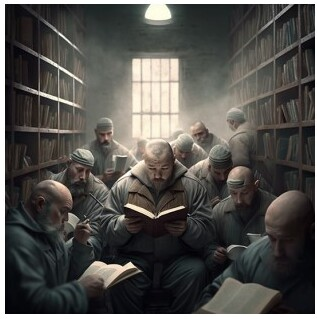
\includegraphics[width=\textwidth,height=0.85\textheight,keepaspectratio]{51.jpg}
			\caption{A large cell of prisoners reading books}
		\end{figure}
	\end{frame}
	
	\begin{frame}[plain]
		\begin{figure}
			\centering
			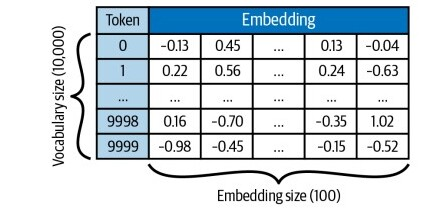
\includegraphics[width=\textwidth,height=0.85\textheight,keepaspectratio]{52.jpg}
			\caption{An embedding layer is a lookup table for each integer token}
		\end{figure}
	\end{frame}
	
	\begin{frame}[plain]
		\begin{figure}
			\centering
			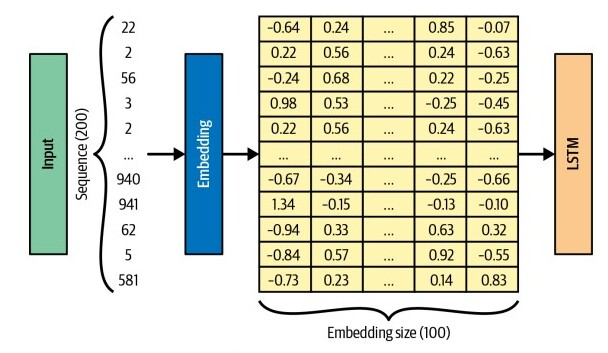
\includegraphics[width=\textwidth,height=0.85\textheight,keepaspectratio]{53.jpg}
			\caption{A single sequence as it flows through an embedding layer}
		\end{figure}
	\end{frame}
	
	\begin{frame}[plain]
		\begin{figure}
			\centering
			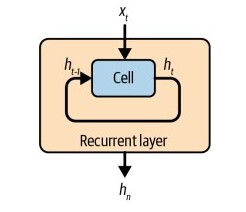
\includegraphics[width=\textwidth,height=0.85\textheight,keepaspectratio]{54.jpg}
			\caption{A simple diagram of a recurrent layer}
		\end{figure}
	\end{frame}
	
	\begin{frame}[plain]
		\begin{figure}
			\centering
			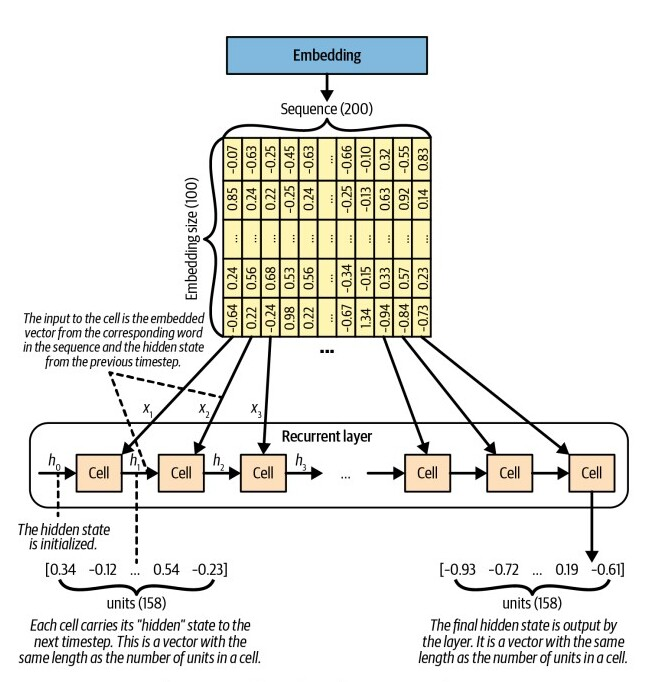
\includegraphics[width=\textwidth,height=0.85\textheight,keepaspectratio]{55.jpg}
			\caption{How a single sequence flows through a recurrent layer}
		\end{figure}
	\end{frame}
	
	\begin{frame}[plain]
		\begin{figure}
			\centering
			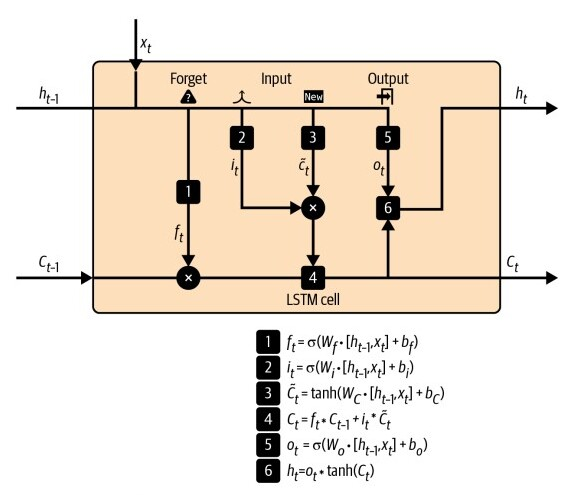
\includegraphics[width=\textwidth,height=0.85\textheight,keepaspectratio]{56.jpg}
			\caption{An LSTM cell}
		\end{figure}
	\end{frame}
	
	\begin{frame}[plain]
		\begin{figure}
			\centering
			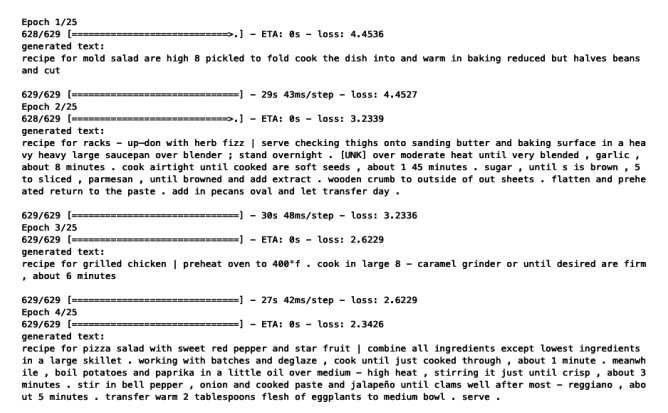
\includegraphics[width=\textwidth,height=0.85\textheight,keepaspectratio]{57.jpg}
			\caption{The first few epochs of the LSTM training process}
		\end{figure}
	\end{frame}
	
	\begin{frame}[plain]
		\begin{figure}
			\centering
			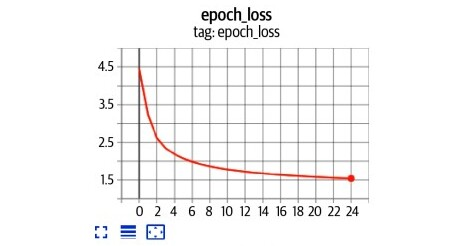
\includegraphics[width=\textwidth,height=0.85\textheight,keepaspectratio]{58.jpg}
			\caption{The cross-entropy loss metric of the LSTM training process by epoch}
		\end{figure}
	\end{frame}
	
	\begin{frame}[plain]
		\begin{figure}
			\centering
			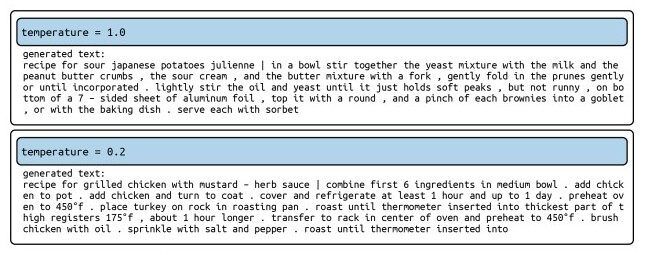
\includegraphics[width=\textwidth,height=0.85\textheight,keepaspectratio]{59.jpg}
			\caption{Generated outputs at temperature = 1.0 and temperature = 0.2}
		\end{figure}
	\end{frame}
	
	\begin{frame}[plain]
		\begin{figure}
			\centering
			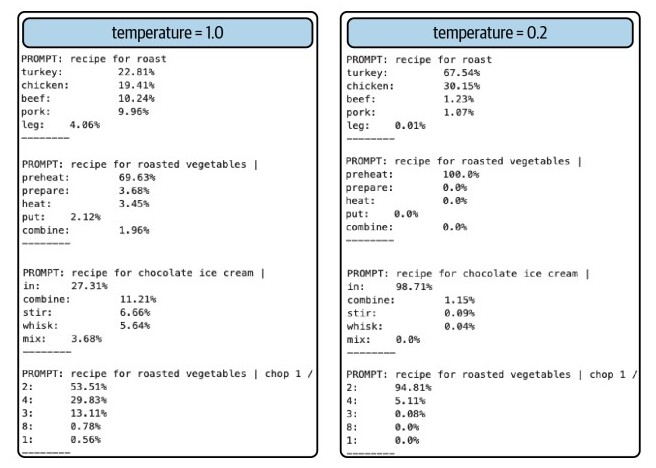
\includegraphics[width=\textwidth,height=0.85\textheight,keepaspectratio]{510.jpg}
			\caption{Distribution of word probabilities following various sequences, for tempera‐
				ture values of 1.0 and 0.2}
		\end{figure}
	\end{frame}
	
	\begin{frame}[plain]
		\begin{figure}
			\centering
			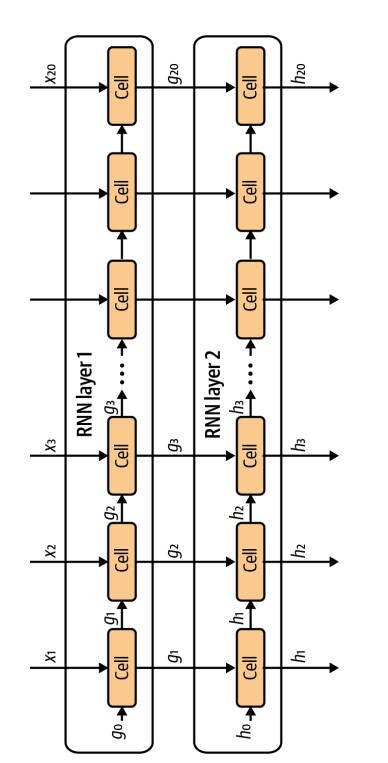
\includegraphics[width=\textwidth,height=0.85\textheight,keepaspectratio]{511.jpg}
			\caption{Diagram of a multilayer RNN: gt denotes hidden states of the first layer and ht denotes hidden states of the second layer}
		\end{figure}
	\end{frame}
	
	\begin{frame}[plain]
		\begin{figure}
			\centering
			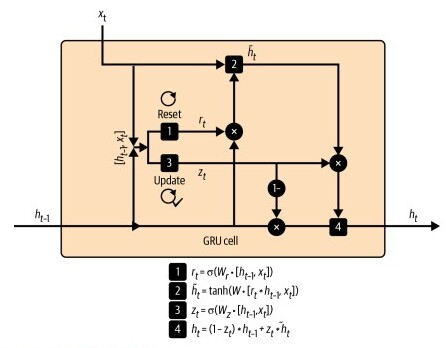
\includegraphics[width=\textwidth,height=0.85\textheight,keepaspectratio]{512.jpg}
			\caption{A single GRU cell}
		\end{figure}
	\end{frame}
	
	\begin{frame}[plain]
		\begin{figure}
			\centering
			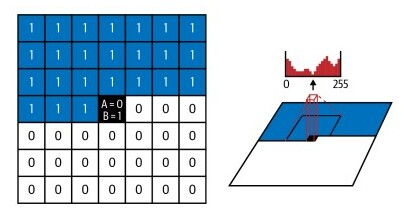
\includegraphics[width=\textwidth,height=0.85\textheight,keepaspectratio]{513.jpg}
			\caption{Left: a convolutional filter mask; right: a mask applied to a set of pixels to
				predict the distribution of the central pixel value}
		\end{figure}
	\end{frame}
	
	\begin{frame}[plain]
		\begin{figure}
			\centering
			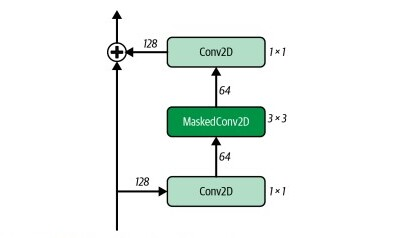
\includegraphics[width=\textwidth,height=0.85\textheight,keepaspectratio]{514.jpg}
			\caption{A PixelCNN residual block (the numbers of filters are next to the arrows
				and the filter sizes are next to the layers)}
		\end{figure}
	\end{frame}
	
	\begin{frame}[plain]
		\begin{figure}
			\centering
			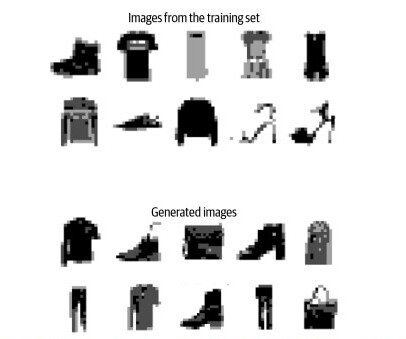
\includegraphics[width=\textwidth,height=0.85\textheight,keepaspectratio]{515.jpg}
			\caption{Example images from the training set and generated images created by the
				PixelCNN model}
		\end{figure}
	\end{frame}
	
	\begin{frame}[plain]
		\begin{figure}
			\centering
			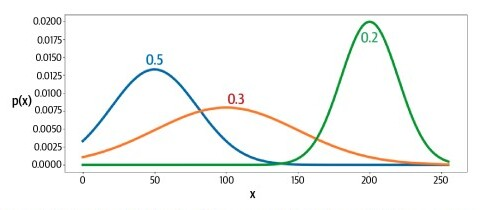
\includegraphics[width=\textwidth,height=0.85\textheight,keepaspectratio]{516.jpg}
			\caption{A mixture distribution of three normal distributions with different parame‐
				ters—the categorical distribution over the three normal distributions is [0.5, 0.3,
				0.2]}
		\end{figure}
	\end{frame}
	
	\begin{frame}[plain]
		\begin{figure}
			\centering
			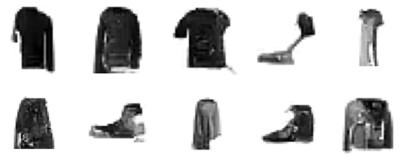
\includegraphics[width=\textwidth,height=0.85\textheight,keepaspectratio]{517.jpg}
			\caption{Outputs from the PixelCNN using a mixture distribution output}
		\end{figure}
	\end{frame}
	
\end{document}